\documentclass[a4paper, 11pt]{article}
\usepackage[margin=1in]{geometry}
\usepackage[polish]{babel}
\usepackage[T1]{fontenc}
\usepackage[utf8]{inputenc}
\usepackage{hyperref}
\usepackage{array}
\usepackage{amssymb}
\usepackage{amsmath}
\usepackage{listings}
\hypersetup{
    colorlinks,
    citecolor=black,
    filecolor=black,
    linkcolor=black,
    urlcolor=black
}
\usepackage{graphicx}

\usepackage{tikz}
\usetikzlibrary{fit,arrows,matrix,positioning, calc, shapes.gates.logic.IEC, shapes.gates.logic.US,arrows,arrows.meta}
\tikzstyle{branch}=[fill,shape=circle,minimum size=3pt,inner sep=0pt]

\definecolor{codegreen}{rgb}{0,0.6,0}
\definecolor{codegray}{rgb}{0.5,0.5,0.5}
\definecolor{codepurple}{rgb}{0.58,0,0.82}
\definecolor{backcolour}{rgb}{0.95,0.95,0.92}

\lstdefinestyle{mystyle}{
    backgroundcolor=\color{backcolour},   
    commentstyle=\color{codegreen},
    keywordstyle=\color{magenta},
    numberstyle=\tiny\color{codegray},
    stringstyle=\color{codepurple},
    basicstyle=\ttfamily\footnotesize,
    breakatwhitespace=false,         
    breaklines=true,                 
    captionpos=b,                    
    keepspaces=true,                 
    numbers=left,                    
    numbersep=5pt,                  
    showspaces=false,                
    showstringspaces=false,
    showtabs=false,                  
    tabsize=4
}

\lstset{style=mystyle}

\title{%
        % \vspace{-3.5cm}
       \large Sprawozdanie Laboratorium PTC \\
       \huge Realizacja układów cyfrowych z wykorzystaniem FPGA}

\author{Stanisław Fiedler 160250, L1}
\date{LAB 5, 2 grudnia 2024}

\begin{document}

\maketitle
%\tableofcontents

\section{Tresc zadania}\label{sec:tresc_zadania} % (fold)
Korzystając z Xilinx ISE dokonaj implementacji transkodera 4x4.
\begin{description}
	\item[a.] Z tabeli 1 wybierz wariant odpowiadający ostatniej cyfrze Twojego numeru indexu.
	\item[b.] Opisz układ w języku VHDL.
	\item[c.] Zaimplementuj układ korzystając z Xilinx ISE
	\item[d.] Wykonaj symulację układu korzystając z ISim
\end{description}
% section Tresc zadania (end)
Wariant:
\vspace{0.3cm}

\begin{tabular}{l|llllllllllllllll}
	wejscie & 0 & 1 & 2 & 3 & 4 & 5 & 6 & 7 & 8 & 9 & A & B & C & D & E & F \\
	\hline
	wyjście & 1 & E & B & F & - & C & 0 & A & - & 4 & 7 & D & 6 & 3 & 5 & 9
\end{tabular}

\section{Plik VHD}\label{sec:plik_vhd} % (fold)
\lstinputlisting{../vhd.txt}
% section Plik VHD (end)

\section{Plik UCF}\label{sec:plik_ucf} % (fold)
\lstinputlisting{../ucf.txt}
% section Plik UCF (end)

\section{Plik testbench}\label{sec:plik_testbench} % (fold)
\lstinputlisting[firstline=28]{../tb_vhd.txt}
% section Plik testbench (end)

\section{Wyniki symulacji}\label{sec:wyniki_symulacji} % (fold)

\begin{center}
	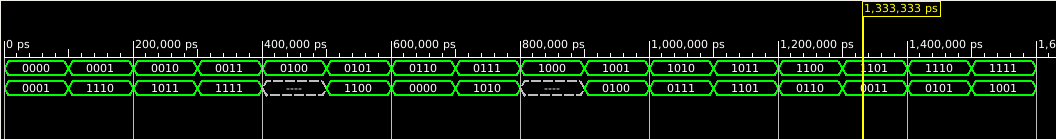
\includegraphics[scale=0.6]{images/symulacja.png}
\end{center}
% section Licznik modulo 12 (end)

\end{document}
